%
%  This simple example illustrates how documents can be
%  split into smaller segments, each segment processed
%  by latex2html separately.  This document can be
%  processed through latex and latex2html with the
%  corresponding makefile.
%

\documentclass{article}         % Must use LaTeX 2e
\usepackage[plainpages=false, colorlinks=true, citecolor=black, filecolor=black, linkcolor=black, urlcolor=black]{hyperref}		
\usepackage[left=.75in,right=.75in,top=.75in,bottom=.75in]{geometry}
\usepackage{makeidx,color,boxedminipage}
\usepackage{graphicx,float}
\usepackage{amsmath,amsthm,amsfonts,amscd,amssymb} 

%%%%%%%%%%%%%%%%%%%%%%%%%%%%%%%%%%%%%%%%%%%%%%%%%%%%%%%%%%%%%%%%%%%%%%
%	Some math support.					     %
%%%%%%%%%%%%%%%%%%%%%%%%%%%%%%%%%%%%%%%%%%%%%%%%%%%%%%%%%%%%%%%%%%%%%%
%
%	Theorem environments (these need the amsthm package)
%
%% \theoremstyle{plain} %% This is the default

\newtheorem{thm}{Theorem}[section]
\newtheorem{cor}[thm]{Corollary}
\newtheorem{lem}[thm]{Lemma}
\newtheorem{prop}[thm]{Proposition}
\newtheorem{ax}{Axiom}

\theoremstyle{definition}
\newtheorem{defn}{Definition}[section]

\theoremstyle{remark}
\newtheorem{rem}{Remark}[section]
\newtheorem*{notation}{Notation}
\newtheorem*{exrcs}{Exercise}
\newtheorem*{exmple}{Example}

%\numberwithin{equation}{section}


%%%%%%%%%%%%%%%%%%%%%%%%%%%%%%%%%%%%%%%%%%%%%%%%%%%%%%%%%%%%%%%%%%%%%%
%	Macros.							     %
%%%%%%%%%%%%%%%%%%%%%%%%%%%%%%%%%%%%%%%%%%%%%%%%%%%%%%%%%%%%%%%%%%%%%%
%
%	Here some macros that are needed in this document:

\newcommand{\motion}{\mathbf{\varphi}}
\newcommand{\hmotion}{\mbox{\boldmath $\hat{\varphi}$}}
\newcommand{\cauchy}{\mbox{\boldmath $\sigma$}}
\newcommand{\eqn}[1]{(\ref{#1})}
\newcommand{\hOmega}{\hat{\Omega}}
\newcommand{\homega}{\hat{\omega}}
\newcommand{\nphalf}{n+\frac{1}{2}}
\newcommand{\nmhalf}{n-\frac{1}{2}}
\newcommand{\kmhalf}{k-\frac{1}{2}}
\newcommand{\kphalf}{k+\frac{1}{2}}
\newcommand{\picdir}{pdffig/}

\title{Advanced Appliations of Synthetic MR and MAGiC}
\author{}
\begin{document}                % The start of the document
\maketitle


%%%%%%%%%%%%%%%%%%%%%%%%%%%%%%%%%%%%%%%%%%%%%%%%%%%%%%%%%%%%%%%%
\section{Physics Model}\label{PhysicsModel}
%%%%%%%%%%%%%%%%%%%%%%%%%%%%%%%%%%%%%%%%%%%%%%%%%%%%%%%%%%%%%%%%
The steady-state magnetization $M_{TD}$ at a specific delay time $T_D$ can be found as a function of flip angle $\theta$, repetition time $T_R$, excitation pulse $\alpha$, and relaxation time  $T_1$:
\[
  M_{TD}  =  M_0\frac{1-(1-\cos(\theta))e^{-\frac{T_D}{T_1}}-\cos(\theta)e^{-\frac{T_R}{T_1}}}{1-\cos(\theta)e^{-\frac{T_R}{T_1}}\cos(\alpha)}
\]
where, $M_0$ is the unsatuarated magnetization.
%%%%%%%%%%%%%%%%%%%%%%%%%%%%%%%%%%%%%%%%%%%%%%%%%%%%%%%%%%%%%%%%
\section{Mathematical Framework}\label{GeneralMathFramework}
%%%%%%%%%%%%%%%%%%%%%%%%%%%%%%%%%%%%%%%%%%%%%%%%%%%%%%%%%%%%%%%%

The underlying philosophy and assumptions within our approach is that the physics 
models are 1st order accurate or within 70-80\% of the needed accuracy and the error is
adequate within the assumed Gaussian noise.
Gaussian distributions provide analytical representations of the random
variables of interest (ie T1, T2) within the Bayesian setting and 
provide a crux for understanding. In particular, we say that a random
variable $\eta$ belongs to a multi-variate normal distribution 
of mean $\mu \in \mathbb{R}^n $ and covariance $\Sigma \in \mathbb{R}^{n \times n}$
\[
     \eta \sim \mathcal{N}(\mu,\Sigma)  
    \Rightarrow
      p(\eta)  = \frac{1}{2 \; \pi \; \det{\Sigma}} \exp\left( - \frac{1}{2} \| \mu - \eta\|^2_{\Sigma}\right)
\]


\begin{enumerate}
  \item Our data acquistion model, $\mathcal{G}(\vec{k},\theta): \mathbb{R}^a
\times \mathbb{R}^m \rightarrow \mathbb{R}^n $,
maps deterministic acquisition
parameters, $\vec{k} \in \mathbb{R}^a$, and uncertain parameters, $\theta \in \mathbb{R}^m$
to observables, $\vec{z} \in \mathbb{R}^n$ ( or $\vec{z} \in \mathbb{C}^n$).
Explicitly, we will assume that the
measurement models are corrupted by zero mean white noise noise of a
\textbf{known} covariance matrix, $\Sigma_z \in \mathbb{R}^{n \times n}$ 
\begin{equation}
\label{sensormodelstructure}
\begin{split}
  \vec{z} & = \mathcal{G}(\vec{k};\theta) + \eta   \qquad   \eta \sim \mathcal{N}(0,\Sigma_z)
      \\
  \vec{k} & =  \text{(TE, TR, etc)}
      \\
  \theta &  =  \text{(T1, T2, etc)}
     \end{split}
\end{equation}
$\eta$ may be interpreted as the measurement noise or the acquisition noise
in the sensor model. For a deterministic measurement model $\mathcal{G}$,
the conditional probablity distribution has an explicit analytical form
and may be written as a  \textbf{known} Gaussian
distribution. 
  \[ 
      p(\vec{z}|\theta)   =  \mathcal{N}(\mathcal{G}(\vec{k};\theta),\Sigma_z)  
  \]
  \item Additional \textbf{known} information is the prior probability
distributions for the model parameters, $p(\theta)$.  For simplicity,
    assume that Prior parameters are Gaussian distributed of 
   \textbf{known} mean, $\hat{\theta}$ and covariance, $\Sigma_\theta$
   \[
      \theta \sim \mathcal{N} (\hat{\theta}, \Sigma_\theta)
   \]
  \item Bayes theorem is fundamental to the approach.
The probability of the measurements $p(z)$ must be interprited in terms of the
known information. The probability of the measurements may be derived from
the marginalization of the joint probability and has the interpretation as
the projection of the joint probability onto the measurement axis.
\[
  p(z) = \int_\theta p(\theta,z)  \; d\theta 
       = \int_\theta p(z|\theta) \; p(\theta)\; d\theta 
\]
  \item  The concept of informational entropy~\cite{Madankan15}, $H(Z)$,
provides a mathematically rigorous framework to look for measurement acquisition
parameters, $\vec{k}$, with the high information content of the reconstruction.
Given a probability space 
$(\Omega, \mathcal{F},p)$ (probability maps from the
sigma-algebra of possible events $p:\mathcal{F}\rightarrow [0,1]$
sigma-algebra, $\mathcal{F}$, defined on set of `outcomes' $\Omega$
\cite{durrett2010probability}),
we will define information of an event  as
proportional to the inverse probability.
\[
\text{information} \equiv  \frac{1}{p(z)}
\]
Intuitively, when a low probability event occurs this provides high
information.
The informational entropy is an \textit{average}
of the information content for a sigma algebra of events $\mathcal{F}$
\[
H(Z) = \int_Z  p(z) \ln\frac{1}{p(z)} \; dz
\qquad
  p(z) = \int_\theta p(z|\theta) \; p(\theta)\; d\theta 
\]
Hence this entropy measure is an average of the information content
for a given set of events, $\mathcal{F}$, and is proportional to the
variance or uncertainty in which the set of events occur.
This agrees with thermodynamic entropy;
if the information containing events are completely spread out such as in a
uniform distribution, the entropy is maxmized.
The entropy
is zero for a probability distribution in which
only one event occurs. Zero information is gained when the same event
always occurs ($0 \ln\frac{1}{0} = 0$). 
Intuitively, we want to find acquisition parameters,
$\vec{k}$, for which the measurements are most uncertain
\[
\max_k H(Z)
  \quad \Leftrightarrow \quad
\min_k 
    \int_Z   dz \underbrace{\int_\theta  d\theta \; p(z|\theta) \; p(\theta)}_{p(z)}
                \underbrace{ln \left(\int_\theta  d\theta \; p(z|\theta) \; p(\theta)\right)}_{ln \; p(z)}
\]
Alternatively we may consider this entropy maximization problem as a
sensitivity analysis for the variance of the measurement $Z$, ie . 
$ \max_k H(Z) \approx  \max_k \text{Var}(Z) $
\[ \begin{split}
   \bar{Z} = \mathbb{E}[Z]  & = \int_Z   dz \; z
   \underbrace{\int_\theta  d\theta \; p(z|\theta) \; p(\theta)}_{p(z)}
  \\
   \mathbb{E}[ ( Z - \bar{Z} )^2 ]  & = \int_Z   dz \;(z - \bar{Z})^2 
   \underbrace{\int_\theta  d\theta \; p(z|\theta) \; p(\theta)}_{p(z)}
  \\
   &  \propto
    \int_Z   dz \;(z - \bar{z})^2 \int_\theta  d\theta 
 \exp\left( - \frac{1}{2} \|  z- \mathcal{G}(\vec{k},\theta)  \|^2_{\Sigma_z}\right)
 \exp\left( - \frac{1}{2} \|  \theta - \hat{\theta}  \|^2_{\Sigma_\theta}\right)
 \end{split}
\]
Probilistic integrals may be
computed from uncertainty quantification
techniques~\cite{fahrenholtz2013generalised}.

 

\end{enumerate}

%%%%%%%%%%%%%%%%%%%%%%%%%%%%%%%%%%%%%%%%%%%%%%%%%%%%%%%%%%%%%%%%
\section{WIP - Echo train length }\label{ModelFidelity}
%%%%%%%%%%%%%%%%%%%%%%%%%%%%%%%%%%%%%%%%%%%%%%%%%%%%%%%%%%%%%%%%


% http://mriquestions.com/fse-parameters.html
% http://mriquestions.com/what-is-fsetse.html

In conventional spin-echo imaging, two basic timing parameters are
required, repetition time (TR) and echo time (TE), Figure~\ref{fig:echotrain}(a).
Similar to
fast spin echo (FSE) imaging, 
the acquistion is setup to acquire multiple lines of k-space in a single TR.
In this situation,
TE is replaced by effective echo
time  and addition parameters are needed: 

\begin{itemize}
\item TE$_\text{eff} \equiv$ the time at which the central lines of k-space are being filled.
\item Number of echoes $\equiv$ called echo train length (ETL)
\item Time between echoes $\equiv$ called echo spacing (ESP) 
\end{itemize}



\begin{figure}[h] 
\begin{tabular}{ccc}
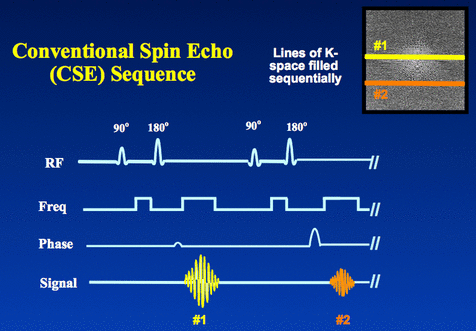
\includegraphics[width=.3\textwidth]{\picdir/7162303.png}
&
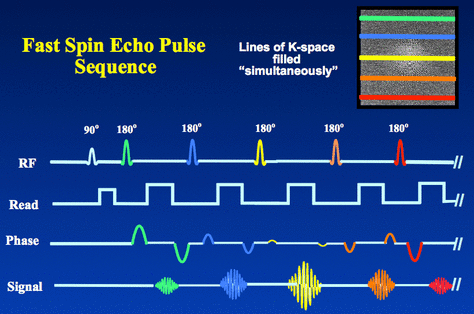
\includegraphics[width=.3\textwidth]{\picdir/5013564.png}
&
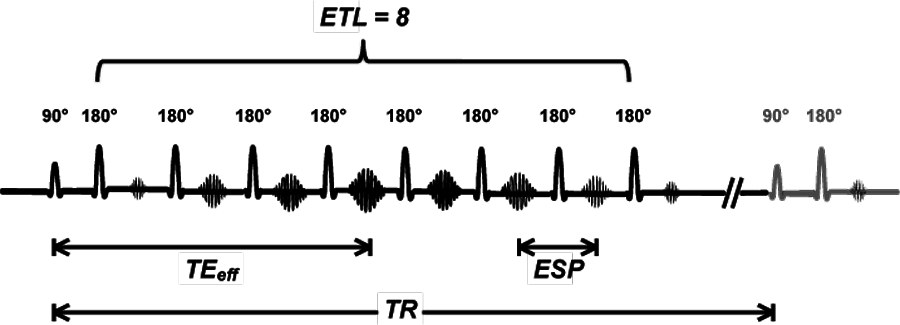
\includegraphics[width=.3\textwidth]{\picdir/3316708_orig.png}
\\
(a) & (b) & (c) \\
\end{tabular}
\caption{ 
(a)
}\label{fig:echotrain}
\end{figure}


{\color{red}
   TODO - need to update signal model for multiple read out lines
}


%%%%%%%%%%%%%%%%%%%%%%%%%%%%%%%%%%%%%%%%%%%%%%%%%%%%%%%%%%%%%%%%
\section{WIP - Inverse Problem Framework}\label{InverseProbFramework}
%%%%%%%%%%%%%%%%%%%%%%%%%%%%%%%%%%%%%%%%%%%%%%%%%%%%%%%%%%%%%%%%
\[
  \vec{z}  = \mathcal{G}(\theta) + \eta   \qquad   \eta \sim \mathcal{N}(0,\Sigma_z)
\]
\[
  p(z|\theta ) = \exp \left( \|\vec{z} -  \mathcal{G}(\theta)\|^2_{\Sigma_z} \right)
\]
\[
               d\left(\vec{z}, \mathcal{G}(\theta^*)\right) = 
   \min_{\theta \in \Omega} d\left(\vec{z}, \mathcal{G}(\theta)\right)
\qquad
\theta = \left(\mu_\text{CSF}, \mu_\text{GM}, \mu_\text{WM}, \mu_\text{Tumor} \right)
\]
%%%%%%%%%%%%%%%%%%%%%%%%%%%%%%%%%%%%%%%%%%%%%%%%%%%%%%%%%%%%%%%%
%%%%%%%%%%%%%%%%%%%%%%%%%%%%%%%%%%%%%%%%%%%%%%%%%%%%%%%%%%%%%%%%
\nocite{*}
\bibliographystyle{apalike}
\bibliography{references}

\appendix
\section{Bayes - An intuitive example}
Bayes theorem is fundamental to the approach and is immediately
follows from the definition of conditional probability
\[
\left.
\begin{split}
p(y|x)  \equiv  \frac{p(x,y)}{p(x)}  \\
p(x|y)  \equiv  \frac{p(x,y)}{p(y)} 
\end{split}
\right\}
\Rightarrow
p(y|x) p(x) = p(x,y) = p(x|y) p(y)
\Rightarrow
\hspace{-1in}
\begin{split}
p(y|x)  =\frac{ p(x|y) p(y) }{p(x) } \\
p(x|y)  =\frac{ p(y|x) p(x) }{p(y) } \\
\end{split}
\]

As a concrete example, consider the explicit two dimensional joint Gaussian
distribution as a medium for understanding. Here we have two random
variables $\mathbf{x}_1$ and $\mathbf{x}_2$ defined on the same probability
space, $\Omega$.
\[
\mathbf{x}_i: \Omega \rightarrow \mathbb{R}
\qquad
P\left( \left\{ \omega: 
\mathbf{x}_i (\omega) \in A
 \right\}\right)
=
\int_A p(\eta_i) d\eta_i
\]
Intuitively, if we are \textbf{given} the joint distribution,
$p(\eta_1,\eta_2)$, knowledge of the realization of one particular random
variable provides information on the realization of the second random
variable.
\[
      p(\eta_1,\eta_2)  = \frac{1}{2 \; \pi \; \sqrt{\det{\Sigma}}}
\exp\left( \frac{1}{2}
\begin{bmatrix}
\eta_1 - \mu_1 \\
\eta_2 - \mu_2 \\
\end{bmatrix}^\top
\underbrace{
\begin{bmatrix}
       \sigma_1^2        & r_{12} \sigma_1 \sigma_2 \\
r_{12} \sigma_1 \sigma_2 &          \sigma_2^2 \\
\end{bmatrix}
}_{\equiv \Sigma}
\begin{bmatrix}
\eta_1 - \mu_1 \\
\eta_2 - \mu_2 \\
\end{bmatrix}
\right)
\]

See \cite{maybeck1979stochastic} (Sec 3.10), characteristic functions 
are used to show that individual marginal
densities of joint  Gaussian random variable is also Gaussian.
\[
p(\eta_1) = 
\int_{\eta_2}
      p(\eta_1,\eta_2)
\;d\eta_2
 = \frac{1}{ \sqrt{2 \; \pi \; \sigma_2^2}} \exp\left( - \frac{(\eta_1 -
\mu_1)^2}{2 \sigma_1^2} \right)
\]

\[
p(\eta_2) = 
\int_{\eta_1}
      p(\eta_2,\eta_1)
\;d\eta_1
 = \frac{1}{ \sqrt{2 \; \pi \; \sigma_1^2}} \exp\left( - \frac{(\eta_2 -
\mu_2)^2}{2 \sigma_2^2} \right)
\]

Conditional probablity is \textit{defined} through the algegraic
reduction of the ratio of the joint and the marginal densities
\[
p(\eta_1|\eta_2) =  \frac{p(\eta_1,\eta_2)  }{p(\eta_2) }
 = \frac{1}{ \sqrt{2 \; \pi \; \sigma_{1|2}^2}}
    \exp\left( - \frac{(\eta_1 - \mu_{1|2})^2}{2 \sigma_{1|2}^2} \right)
 = 
\frac{p(\eta_1)}{p(\eta_2)}
   \frac{1}{ \sqrt{2 \; \pi \; \sigma_{2|1}^2}}
    \exp\left( - \frac{(\eta_2 - \mu_{2|1})^2}{2 \sigma_{2|1}^2} \right)
\]
\[
\mu_{1|2} =  \mu_1 - 
       \frac{r_{12} \sigma_1 \sigma_2 }{\sigma_2^2}
       (\eta_2 - \mu_2)
\qquad
\sigma_{1|2} = 
\sigma_1^2  - 
       \frac{(r_{12} \sigma_1 \sigma_2 )^2}{\sigma_2^2}
\]
\[
\mu_{2|1} =  \mu_2 - 
       \frac{r_{12} \sigma_1 \sigma_2 }{\sigma_1^2}
       (\eta_1 - \mu_1)
\qquad
\sigma_{2|1} = 
\sigma_2^2  - 
       \frac{(r_{12} \sigma_1 \sigma_2 )^2}{\sigma_1^2}
\]

\end{document}
